\subsection{Cosmic rays}
\begin{figure}[h!]
    \centering
    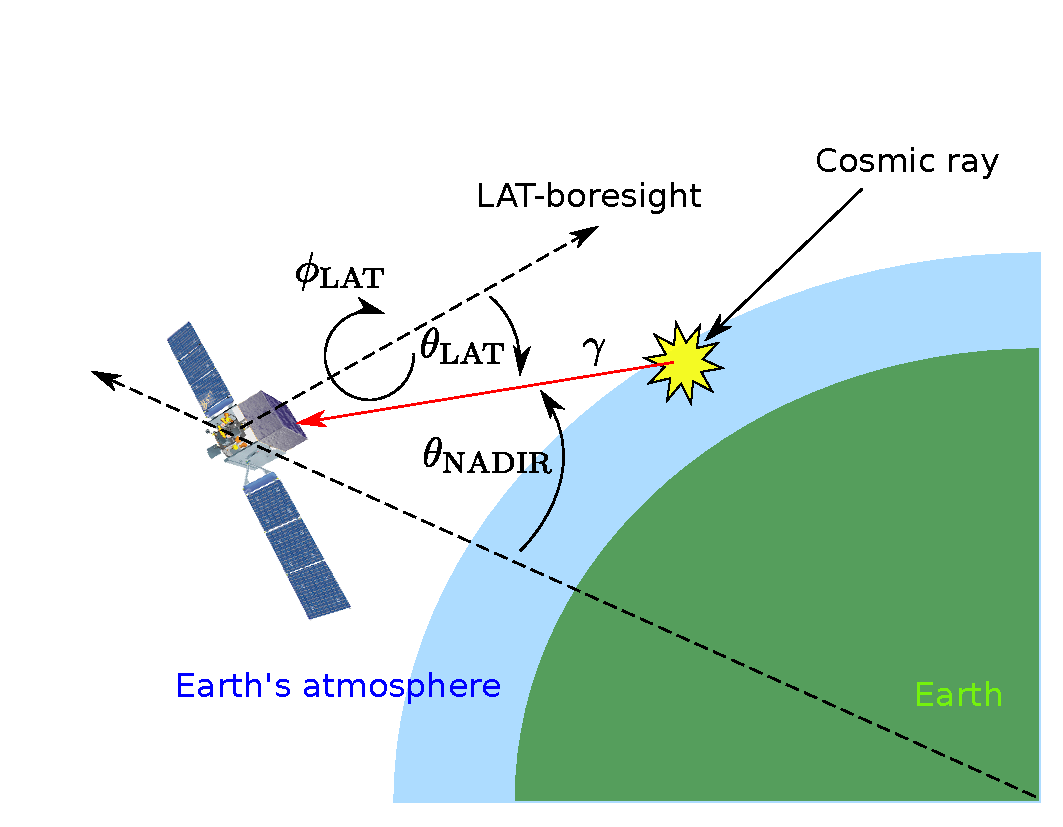
\includegraphics[width=0.7\textwidth]{img/gamma_production_schematic}
    \caption{Schematic of $\gamma$-ray production}
\end{figure}
Cosmic rays (CRs) are high energy particles which are produced in space by various types
of acceleration mechanisms such as supernovae, active galactic nuclei, quasars, and
gamma-ray bursts. The main composition of CRs consist of 90\% protons, 8\% alpha
and other heavier atoms.
The widely accepted explanation of why CR spectrum follows a power-law function in rigidity is that the acceleration mechanism was modeled as a diffusive shock which has a characteristic spectral index.
% The main reason that makes CRs spectrum follow power
% law function in rigidity is the acceleration mechanisms in space was dominated in
% Lorenzian interaction which has a characeteristic spectral index.

\par The values of CR spectral indices vary for different ranges of energies, depending on the types of sources which can accelerate CRs to a certain energy range as shown in Figure \ref{fig:cr_overview_spectrum} and Figure \ref{fig:cr_famous_spectrum} \cite{Swordy2001}.

\begin{figure}[h!]
  \centering
  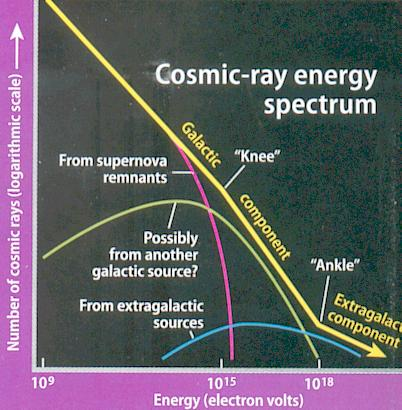
\includegraphics[width=0.6\textwidth]{img/cr_feature_ref_university-review_ca}
  \caption{characeteristic of CRs spectrum: Image taken from universe-review.ca}
  \label{fig:cr_overview_spectrum}
\end{figure}
\begin{figure}[h!]
    \centering
    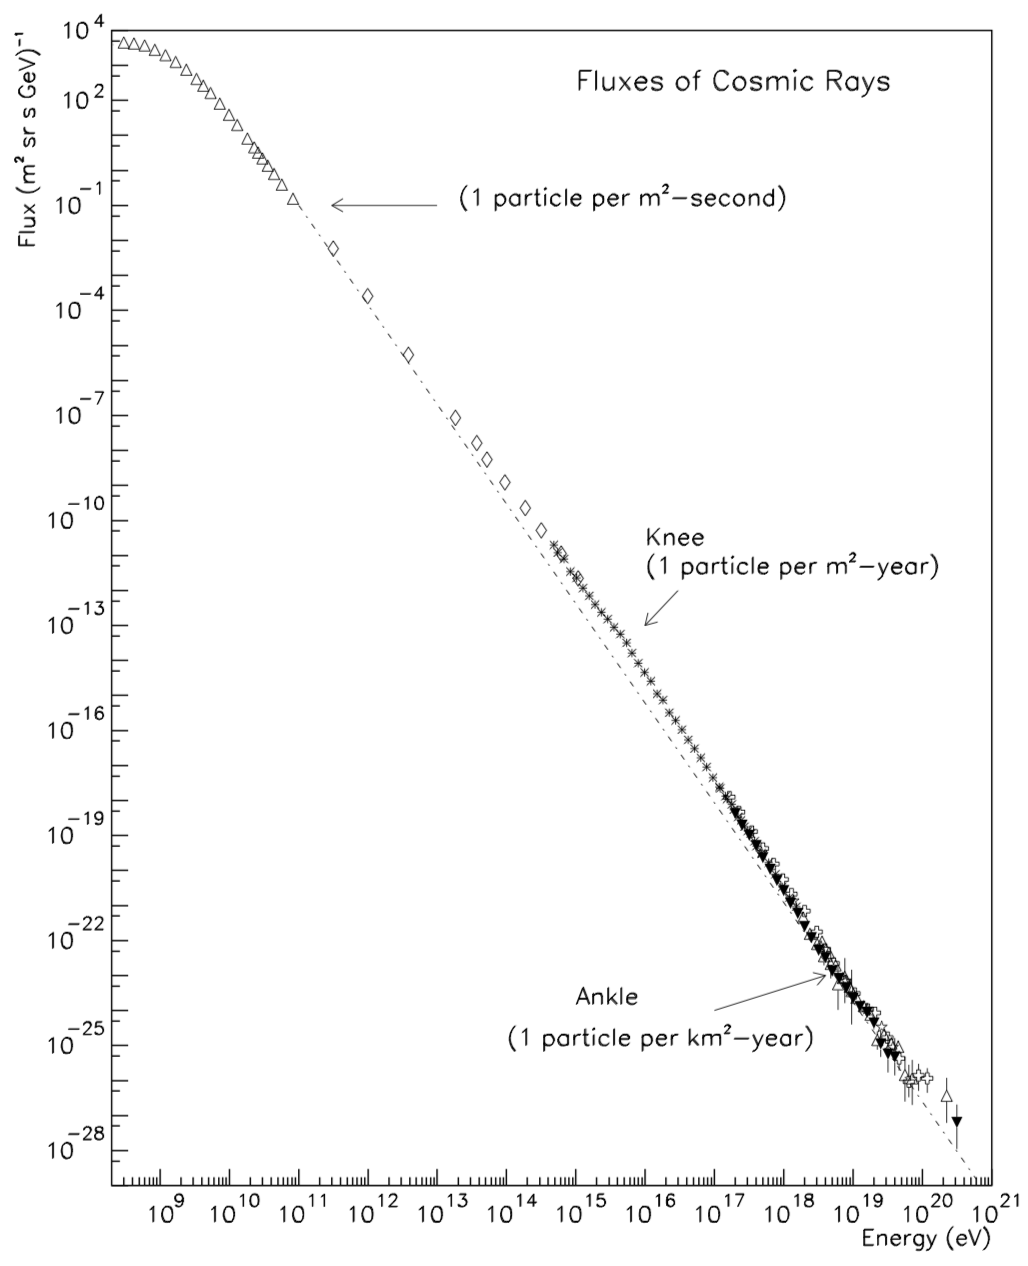
\includegraphics[width=0.6\textwidth]{img/Swordy}
    \caption{Observation of CRs spectrum: Image taken from \citet{Swordy2001}}
    \label{fig:cr_famous_spectrum}
\end{figure}

\par The motivation why we use $\gamma$-ray as a secondary product for investigating incident proton spectrum is that Earth limb's $\gamma$-ray relatively brighter than the sky due to collision from CRs in energy range 100 MeV and 1 TeV which consistent with our study \cite{Warit2009}.

\par Previous work has been performed using Pass 7 version data \cite{FermiPass7} and found an energy breakpoint around 300 GeV with a significance level of around 2$\sigma$ \cite{previouswork}. This result agree to the direct measurements from \cite{AMS-02,PAMELA}.


\subsection{\textit{Fermi} Large Area Telescope}

Gamma-ray Large Area Space Telescope (GLAST) could be informally called \textit{Fermi}-LAT. The mission is to collect data of particles from multiple phenomena such as active galaxy nuclei (AGN), pulsars and other high energy sources.
It also attaches the Gamma-ray Burst Monitor (GBM) to study gamma-ray bursts. Fermi was launched on 11 June 2008 at 16:05 UTC aboard a Delta II 7920-H rocket.


\subsubsection*{Instrument}
LAT consists of 16 layers of tracker (TKR) modules, 16 calorimeters (CAL) and a partition Anti-Coincidence Detector (ACD). 

\begin{figure}[h!]
  \centering
    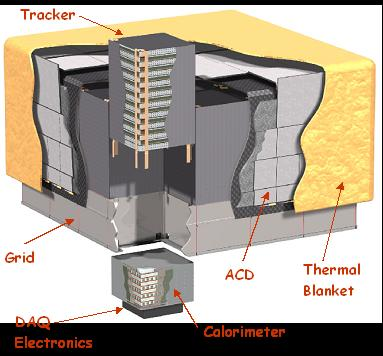
\includegraphics[width=0.5\textwidth]{img/LATStructure}
    \caption{Instrument structure : Image taken from https://fermi.gsfc.nasa.gov}
\end{figure}

\par TKR module has made from an array of silicon-strip tracking detectors (SSDs) and has 18 trackers on a horizontal plane. First 12 planes have 0.035 radiation lengths, next 4 layers contain 0.18 radiation lengths thick and the rest of it does not have any converter.
Tracking detectors in each plane consist of two planar inner layer which running in x and y axis subsequently. The arrival $\gamma$-ray in LAT's field of view could produce electron-positron pair in TKR's plates.
The initial lepton pair could be determined from the record of conversion point in SSD planes with a power angular resolution when it has a low energy.

\par Each CAL module contains 1536 CsI(Tl) crystal with a 96 crystal align in eight different orthogonal layers.
Dual PIN photodiodes also attach in each crystal which provides a great resolution in energy.

\par ACD tile contains wavelength shifting fiber by photomultiplier tubes (PMT) for avoding majoirity of incoming charged particles
to prevent a veto signal in calorimeters which cause an inefficient of the instrument. 

\subsubsection*{Event reconstruction}
The methodology of detection is to track a lepton pair product from an incident photon that collides with the conversion foil and lepton products be traced by the second inner layer of TKR.
Consequently, the limit of precision depends on the energy of photon that larger than the rest mass energy of electron-positron as well as angle resolution of TKR that getting worse at larger $\theta_\text{LAT}$.
Lastly, the energy of the lepton product could be captured by a precision crystal array in CAL. The event classification is divided into various levels of confident \cite{FermiDetail,Atwood:2013rka}.


\begin{figure}[h!]
  \centering
    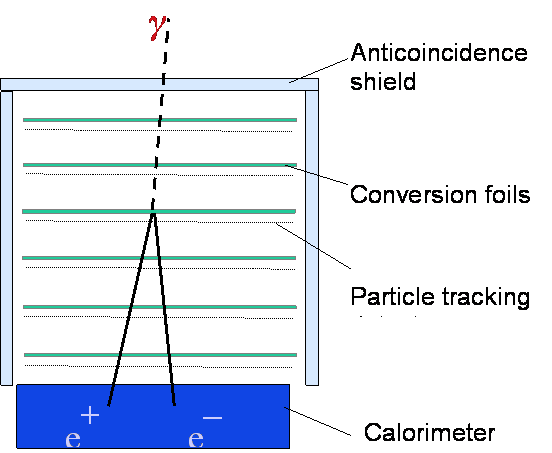
\includegraphics[width=0.5\textwidth]{img/LATMethodology}
    \caption{Structure of the LAT : Image taken from https://fermi.gsfc.nasa.gov}
  \end{figure}
